% arara: xelatex
% arara: xelatex
% arara: xelatex

% options:
% thesis=B bachelor's thesis
% thesis=M master's thesis
% czech thesis in Czech language
% english thesis in English language
% hidelinks remove colour boxes around hyperlinks

\documentclass[thesis=M,english]{prefs/FITthesis}[2019/03/06]

% \usepackage{subfig} %subfigures
% \usepackage{amsmath} %advanced maths
% \usepackage{amssymb} %additional math symbols

\usepackage[utf8]{inputenc}

\usepackage{graphicx} %graphics files inclusion
% \usepackage{amsmath} %advanced maths
% \usepackage{amssymb} %additional math symbols

\usepackage{dirtree} %directory tree visualisation
\usepackage{subfig} %image side by side
\usepackage{todonotes} %todo
\usepackage{url}
\usepackage{textcomp} %degree symbol
\usepackage{color, colortbl} %color, table color
\usepackage{enumitem} %lists
\usepackage{float} %for H option in figures
\usepackage{array} %table aligment       
\usepackage{amsmath} %cases
\usepackage{amssymb}
\usepackage{svg} %svg
\usepackage{scrextend}
\usepackage{multirow}
\usepackage[ruled,vlined]{algorithm2e}
\addtokomafont{labelinglabel}{\sffamily}


\definecolor{LightCyan}{rgb}{0.88,1,1}
\definecolor{Blue}{rgb}{0.30980, 0.50588, 0.73725}
\definecolor{White}{rgb}{1, 1, 1}

% list of acronyms
\usepackage[acronym,nonumberlist,toc,nopostdot,numberedsection=autolabel,nomain]{glossaries}
\makeglossaries
\newcommand{\tg}{\mathop{\mathrm{tg}}} %cesky tangens
\newcommand{\cotg}{\mathop{\mathrm{cotg}}} %cesky cotangens

% % % % % % % % % % % % % % % % % % % % % % % % % % % % % % % % % % % 
% % % % % % % % % % % % % % % % % % % % % % % % % % % % % % % % % % % 
\department{Department of Applied Mathematics}
\title{Vehicle Routing Problem with Time Windows solved via Machine Learning and Optimization Heuristics}
\authorGN{Adam} %author's given name/names
\authorFN{Zvada} %author's surname
\authorWithDegrees{Bc. Adam Zvada} %author's name with academic degrees
\author{Adam Zvada} %author's name without academic degrees
\supervisor{doc. Ing. Pavel Kordík, Ph.D.}
\acknowledgements{TODO}
\abstractCS{TODO}
\abstractEN{TODO}
\placeForDeclarationOfAuthenticity{Prague} %where you have signed the declaration
\keywordsCS{TODO\newpage}
\keywordsEN{TODO}
\declarationOfAuthenticityOption{5} %select as appropriate, according to the desired license

\newacronym{ai}{AI}{artificial intelligence}
\newacronym{vrp}{VRP}{vehicle routing problem}
\newacronym{cvrp}{CVRP}{capacitated vehicle routing problem}
\newacronym{vrptw}{VRPTW}{vehicle routing problem with time windows}
\newacronym{tsp}{TSP}{traveling salesman problem}
\newacronym{ml}{ML}{machine learning}
\newacronym{pdp}{PDP}{Pick and Deliver}
\newacronym{vrppd}{VRPPD}{vehicle routing problem with pick and deliver}
\newacronym{rl}{RL}{reinforcement learning}
\newacronym{mha}{MHA}{Multi-head Attetntion}
\newacronym{gat}{GAT}{Graph Attention Network}
\newacronym{gcn}{GCN}{Graph Convolution Networks}

\newacronym{ctu}{CTU}{Czech Technical University}
\newacronym{cpu}{CPU}{central processing unit}
\newacronym{cv}{CV}{computer vision}
\newacronym{dex}{DEX}{Deep EXpectation}
\newacronym{dl}{DL}{deep learning}
\newacronym{dlt}{DLT}{Direct Linear Transform}
\newacronym{dsae}{DSAE}{deep sparse autoencoders}
\newacronym{fast r-cnn}{Fast R-CNN}{fast region-based convolutional network}
\newacronym{faster r-cnn}{Faster R-CNN}{faster region-based convolutional network}
\newacronym{fce}{FCE}{Faculty of Civil Engineering}
\newacronym{fit}{FIT}{Faculty of Information Technology}
\newacronym{fn}{FN}{false negatives}
\newacronym{fp}{FP}{false positives}
\newacronym{fps}{FPS}{frames per second}
\newacronym{gige}{GigE}{Gigabit Ethernet}
\newacronym{gpu}{GPU}{graphics processing unit}
\newacronym{hog}{HOG}{histogram of oriented gradients}
\newacronym{hsv}{HSV}{hue-saturation-value}
\newacronym{idsw}{IDSW}{identity switches}
\newacronym{improlab}{ImproLab}{Image Processing Laboratory}
\newacronym{iou}{IoU}{intersection over union}
\newacronym{lbp}{LBP}{local binary pattern}
\newacronym{lstm}{LSTM}{long short-term memory}
\newacronym{mae}{MAE}{mean absolute error}
\newacronym{ml}{ML}{machine learning}
\newacronym{mlp}{MLP}{multi layer perceptron}
\newacronym{mot}{MOT}{multiple object tracking}
\newacronym{mota}{MOTA}{multiple object tracking accuracy}
\newacronym{motp}{MOTP}{multiple object tracking precision}
\newacronym{mots}{MOTS}{multiple object tracking and segmentation}
\newacronym{mp}{MP}{megapixel}
\newacronym{mtmct}{MTMCT}{multi-target multi-camera tracking}
\newacronym{nms}{NMS}{non-maximum suppression}
\newacronym{nn}{NN}{neural network}
\newacronym{pca}{PCA}{principal component analysis}
\newacronym{r-cnn}{R-CNN}{region-based convolutional network}
\newacronym{reid}{ReID}{re-identification}
\newacronym{rgb}{RGB}{red-green-blue}
\newacronym{roi}{RoI}{region of interest}
\newacronym{rmse}{RMSE}{root-mean-square error}
\newacronym{rnn}{RNN}{recurrent neural network}
\newacronym{rpn}{RPN}{region proposal network}
\newacronym{sdk}{SDK}{software development kit}
\newacronym{sift}{SIFT}{Scale-invariant feature transform}
\newacronym{sort}{SORT}{simple online and real-time tracking}
\newacronym{ssd}{SSD}{single-shot detector}
\newacronym{ssr}{SSR-Net}{Soft Stagewise Regression Network}
\newacronym{surf}{SURF}{Speeded-Up Robust Features}
\newacronym{spp}{SPP}{spatial pyramid pooling}
\newacronym{svm}{SVM}{support vector machine}
\newacronym{yolo}{YOLO}{you only look once}


\begin{document}
    \begin{introduction}

    Detection of people and their subsequent identity preservation in a video sequence (tracking) is a part of a more broader domain task called \gls{mot}. In the basic definition, \gls{mot} tries to estimate the position of the objects from multiple predefined classes, and then maintain their identity through the whole video sequence. 
    
    In most cases, position estimation is done by a component known as the object detector, which predicts the bounding boxes with real-valued confidences of each object class in each video frame. However, the conventional object detector does not guarantee the relationship between objects in consecutive frames. Therefore, it is necessary to extract additional features from each detected object to build the relationship in the sequence of frames. 
    
    The extracted features are mainly based on a visual appearance, movement, and interactions of the object, but complementary information such as camera calibration and known scene parameters can also be incorporated. The subsequent tracking is then achieved by matching detected objects to preserved tracks based on various distance metrics that are calculated between features of the detected objects in a current frame and features of traced objects from previous frames. This approach is also known as online tracking-by-detection which means that only current and previous frame information is available to the tracker, in contrast with offline-based tracking where information from the whole sequence can be used at any time. 
    
    One of the tracking benefits is that we can recover the trajectories of the objects that appeared in the video sequence, based on which we can calculate various spatial statistics that can help us to improve existing processes. For example, statistics about the movement within waiting halls might be helpful for companies to improve their indoor space and arrangement. 
    
    Even though this thesis focuses only on the task of people tracking, we may still apply many principles from more general \gls{mot}. A follow-up step after successfully building the people tracking framework is the extraction of additional class-specific information about people (soft-biometrics). This estimated data can be utilized in many applications from the retail environment; for example, we can utilize them in a retail store where there is the high demand for learning customer trends in specific days and hours, which could be easily achieved by collecting customer information such as age, gender, mood, etc. Other scenarios could be with a personalized advertisement targeted at passers-by in a shopping center or real-time staff alert when senior enters a store to offer immediate assistance. Moreover, we could use this framework to distinguish between customers and employees so we can analyze their interaction or even go further and optimize the distribution of employees around the store.
    
    \section{Motivation}
        \gls{mot} is one of the essential topics in the computer vision field. A large number of surveillance cameras in use has led to strong demand for automatic methods of processing their outputs. For example in the field of crowd image analysis, the scientific challenge is to devise and implement methods for obtaining detailed information about the number, density, movements, and actions involving people observed by a single camera or by a network of cameras.  
        
        Historically, the progress in \gls{mot} field has been limited by the number and size of the available datasets, and it was especially challenging to make comparisons between algorithms if they have been tested on different datasets under widely varying conditions. Thus, the needs of the researchers eventually formed the very first and most known PETS2009 \cite{ferryman2009pets2009} person tracking dataset. However, this dataset is minimalist. There are only three sequences related to the person tracking with ground-truth information, and evaluation metrics were often applied inconsistently, for example involving using different subsets of the available data, different ways of training the models, or differing evaluation scripts \cite{MOTChallenge2015}.
        
        The big break came in the year 2015 when MOTChallenge \cite{MOTChallenge2015} was released with the goal of standardization of quantitative benchmark to address such issues. Not only did they create unified evaluation framework with standardized metrics, but they also created the large-scale dataset with a total of 22 sequences, half for training and a half for testing purpose, with a total of 11286 frames or 996 seconds of video. This benchmark has massively transformed the \gls{mot} field which resulted in severe improvements to existing algorithms. Its popularity can also be expressed in numbers; for example, 99 \gls{mot} tracking algorithms were submitted to the MOT17 challenge \cite{mot16} during the year 2017 and similarly previous years. 
        
        Since the accuracy of existing algorithms is increasing and the price of \gls{gpu} computations is decreasing, new and more challenging datasets are being invented. VisDrone2018 \cite{zhuvisdrone2018} is a current state-of-the-art \gls{mot} dataset with over 260 video clips and more than 2.5 million bounding boxes of various class objects annotated. The frames are captured by several drone-mounted cameras which causes an unusual perspective and makes the dataset even more challenging. 
        
        To this date, there are more than ten large-scale \gls{mot} benchmarks publicly available which demonstrates that this task, especially with objects such as people, vehicles, and bicycles, has enormous attention in the research community and because the datasets are still updated to be more challenging, there are still places to improve. 
        
        The logical extension beyond detection and tracking horizons is the extraction of additional class-specific features. If we would track cars, we could take advantage of estimation of car paint, brand, and type. This information can then be used for various temporal and regional statistics; for example, for estimating the richness of a town by counting luxury-type cars. 
        
        If we take another case, which is the extraction of class-specific features about people, we could estimate attributes such as race, gender, height, mood, hair color, and clothes color. These traits are called soft-biometrics, and they are frequently used in cases where we need to complement primary biometric identifiers, such as fingerprint, palm veins, iris pattern, to provide authentication based on the unique identification of the person. The estimation of any class-specific feature is noisy. Therefore, it is essential to have reliable \gls{mot} framework, so the features are not collected from a single frame, but appropriately calculated from the whole tracking session.
        
        Although soft-biometric characteristics lack the distinctiveness and permanence to recognize an individual uniquely and reliably and can be easily faked, they provide some evidence about the people identity that could be beneficial \cite{wiki:biometrics}. With the use of soft-biometrics, we can differentiate individuals in surveillance video where it is ubiquitous that people are often occluded. In other words, despite the fact they are unable to individualize a subject, they are useful in distinguishing between people, thus maintaining people's identity in a surveillance scene. Another useful utilization is in the retail environment where we can build aggregated statistics such as the number of women between age 25 and 40 visited our store in the morning. If we have such information that in the morning there is 75 \% women of visitors, we could utilize this and adapt the store to be more suitable for women, and therefore we will have a better chance to increase profit.
        
        Last but not least, having an accurate and flawless \gls{mot} framework is crucial for further expansion to popular \gls{mtmct} field, which is the problem of determining who is where at all times given a set of video streams as input. The output of this task is also a set of person trajectories but from a wider area. Person \gls{reid} is a closely related problem in this field. Given a query image of a person, the goal is to retrieve from a database of images taken by different cameras the images where the same person appears. \cite{ristani2016MTMC}
        
    \section{Challenges}
        \gls{mot} field is deeply explored -- many methods have been proposed, and many surveys have been conducted \cite{luo2014multiple, fan2016survey, emami2018machine}. However, it is still considered as not successfully solved computer vision task. In other words, a saturation point has not yet been reached.
        
        \gls{mot} task is an extension of object detection from single images to video sequence. 
        The main challenges when using an object detector for tracking are that the resulting output is unreliable and sparse, i.e., detectors only deliver a discrete set of responses and usually yield false positives and false negatives (missing detections) as shown in Fig \ref{fig:false positive and false negative}. So, in addition to such object detection errors, identity switches are frequent in any \gls{mot} framework (see Fig. \ref{fig:id switch example}). 
    
        \begin{figure}[ht]
          \centering
          \includegraphics[width=0.7\textwidth]{resources/false-positive_and_false_negative.png}
          \caption{Example of false positive and false negative person detection. Source: \cite{yao2012interactive}.}
          \label{fig:false positive and false negative}
        \end{figure}
        
        \begin{figure}[ht]
          \centering
          \includegraphics[width=0.7\textwidth]{resources/tracking_errors.png}
          \caption{Cases illustrating tracker-to-target assignments errors. (a) An ID switch occurs when the mapping switches from the previously assigned red track to the blue one. (b) A track fragmentation is counted in frame 3 because the target is tracked in frames 1 and 2, then interrupts, and then reacquires its ‘tracked’ status at a later point. A new (blue) track hypothesis also causes an ID switch at this point. Source: \cite{MOTChallenge2015}}
          \label{fig:id switch example}
        \end{figure}
        
        ID switches occur when there are two object trajectories are produced for one ground-truth object. Fragmentation occurs when there are two trajectories are produced with a time gap between them for one ground truth object, which implies that detections are missed in several frames. In theory, the robust tracker should handle both of these flaws. It should fill gaps in detections by propagating information from neighboring frames, and it should also filter false positive detections based on the information from previous frames. 
        
        However, it has been found out during multiple object tracking challenges that in practice, it is not entirely so. For example, in \gls{mot} \cite{mot16} dataset from 2016, 18 \% of tracks are not covered by detections at all, and 37 \% percent of tracks are covered only by low confidence of detections. When there is no high-quality detection for particular ground-truth track, then the tracker cannot resolve this problem at all, which implies that tracker usually reduces only false positives and raise false negatives by removing low-confidence detections. Nowadays, many researchers state that a robust object detector is a key to good tracking \cite{mot16, konushin2017, bewley2016simple} and during recent work \cite{luo2014multiple, fan2016survey, DBLP:journals/corr/abs-1903-05625}, it has been shown that modern object detectors can locate object even in complex, crowded scenes. However, false positives have remained frequent. 
        
        If we narrow down to the tracking people, it is even more difficult because they are very dynamic objects. People tend to change position, direction, and posture often, but they also have different height and body proportions. In real-world scenes, long-term occlusions are also frequent. As a result, it is vital for people tracking systems to be flexible so that it can handle as many different situations as possible.  
        
        Lastly, it is a topic from computer vision field where most of the work is done over images represented by matrices. It is well known that working with images is computationally demanding because each change needs to be applied for each pixel and although the image algorithms can be well parallelized, we still need to keep in mind the computation costs. 
    
    \section{Objectives}
        The goal of this thesis is to design and implement a sophisticated framework that could utilize surveillance sequences for people online tracking followed by the extraction of as much data as possible about the people in the scene, which is a three-step process. First, we need effectively and precisely acquire people detections in each frame. Then, we need to utilize a robust tracking algorithm that will maintain people identities. Lastly, gathered data from people tracking sessions must be appropriately processed for useful output statistics.
    
    \section{Assumptions}   
        The detection and tracking of people in surveillance footage is a broad topic. For this reason, the work is limited only to the one static camera watching a known scene. We assume that the captured scene is entirely under our control which means we can make any measurements and calibrate the camera. Moreover, we take into account the requirements for online processing so that the framework can be improved for real-time inference in the future. 
    
    \section{Thesis structure}
        The rest of this thesis is organized as follows. In the first chapter, we present a theoretical background which is crucial for the understanding of solving this task. Chapter 2 is devoted to the related work. Algorithm design and proposals are presented in chapter 3. Implementation details are explained in chapter 4, followed by the evaluation presented in chapter 5. The whole work is wrapped up in the last Conclusion chapter.
    
\end{introduction}
    \chapter{Introduction to Vehicle Routing Problem}\label{introduction_vrp}

    The problem objective of \gls{vrp} is simply finding the shortest route for multiple vehicles to serve all the given set of customers. The shortest route can be differently interpreted based on your minimalization criteria, e.g, traveled distance, time, or a combination of both. It was first proposed by Dantzig and Ramser \cite{truck-dispatching-problem} in 1959, and since then researchers are coming up with different approaches how to solve the problem. 

    \section{Vehicle Routing Problem Definition}
    
    The general \gls{vrp} can be defined as a problem in a complete graph $G=(V,E)$ of finding the optimal permutation $\pi_l = (\pi_0, \cdots, \pi_m)$ of nodes $V$ all starting from a node $v_0$ for given number of paths $k$ which results in minimal traversal cost where $\forall v \in (V \setminus v_0)$ are visited only once. \gls{vrp} is generalization of \gls{tsp} which only has one path.
    
    \begin{figure}[ht]
        \centering
        \includegraphics[width=0.75\textwidth]{resources/intro/vrp-graph.png}
        \caption{Intuitive view of \gls{vrp} instance on left and proposed solution for 5 vehicles on the right \cite{vrp-malaga}}
        \label{fig:vrp-graph}
    \end{figure}
    
    \gls{vrp}s are classified as NP-Hard problems which was proved by Lenstra and Kan \cite{time-complexity-vrp}. It means that in the worst case, adding new nodes, i.e., customers results in an exponential increase of computational complexity.
    
    \subsection{VRP Notation}
    Let's introduce our used notation and its real-world interpretation.
    \begin{itemize}
        \item $G=(V,E)$ is a complete undirected graph
        \begin{itemize}
            \item Network of routes
        \end{itemize}
        \item $v_0$ is the initial node
        \begin{itemize}
            \item A depot
        \end{itemize}
        \item $V^{\prime} = (v_1, \cdots, v_n)$ nodes expect the initial node
        \begin{itemize}
            \item Geographically scattered location of customers
        \end{itemize}
        \item $E = \{(v_i, v_j)| v_i, v_j \in V, i \neq j\}$ with associated weight as a cost $c: E \to \mathbb{N}^+$
        \begin{itemize}
            \item A single route between two locations with associated cost, e.g., distance.
        \end{itemize}
        \item $C$ is a matrix of edge weights indexed by nodes. $c_i_j$ where $i,j \in V$
        \begin{itemize}
            \item Matrix of costs between customers
        \end{itemize}
        \item $R_i \subset V$ is a path that starts and ends at $v_0$. $(r_0 = v_0 \land r_{|R_i|} = v_0)$
        \begin{itemize}
            \item Route visit a subset of customers starting and ending at the depot, it can be referred to it as a delivery plan.
        \end{itemize}
        \item $k$ number of paths
        \begin{itemize}
            \item Number of vehicles
        \end{itemize}
        \item $R = R_1, \cdots, R_k$ is a set of paths
        \begin{itemize}
            \item All routes (delivery plans) for a given instance of \gls{vrp}.
        \end{itemize}
        \item $\pi = (\pi_1, \cdots, \pi_k)$ solution for a given instance of \gls{vrp}.
        \begin{itemize}
            \item Customer locations in visiting order for multiple vehicles.
        \end{itemize}
    \end{itemize}
    
    \textbf{Fesability of \gls{vrp} solution} for \gls{vrp} of routes $R$ is feasible only if each node $V_1$ is visited exactly once.
    
    \textbf{The cost of route $R_i$} which we aim to minimize is the sum of its weights (costs). If we operate in Euclidean space, then it is L2 norm of route locations.
    \begin{equation}
        C(R_i) := \sum_{k = 0}^{|R_i|} c_{r_k}_{r_k+1}
    \end{equation}
    
    \textbf{The cost of \gls{vrp} solution} is the sum of route costs.
    \begin{equation}
        C(R) := \sum_{i = 1}^{|R|} C(R_i)
    \end{equation}
    
\section{Vehicle Routing Flavors}
Our modern world heavily relies on complex logistics networks. It requires to synchronize multimodal planning to ship your goods from one side of the world to your doorstep. In order to achieve this, multiple variants and flavours of \gls{vrp} had to be studied and implemented in the real world use cases. It goes from ordinary variants like measuring the capacity of cars to a more niche problem like eVRP where vehicles are required to make stops to recharge.

All the flavours of \gls{vrp} can be mutually combined, which is usually the main area of research.

    \begin{figure}[ht]
        \centering
        \includegraphics[width=1.0\textwidth]{resources/intro/vrp-flavours.png}
        \caption{Taxonomy of VRPs \cite{bono-stochastic-vrp}}
        \label{fig:vrp-flavours}
    \end{figure}

The sections below are describing each flavour shown in \ref{fig:vrp-flavours}.

    \subsection{Capacitated Vehicle Routing Problem}
    The \gls{cvrp} extends the regular \gls{cvrp} in introducing a capacity element for each customer. In the literature, it is sometimes referred to as a demand. The customer's demand is $d \in \mathbb{N}^+$ which may represent capacity in the form of weight, size but also in some abstract concepts such as a basket of apples. Additionally, each vehicle has a predefined capacity $Q > 0$.
    
    The \gls{cvrp} extends the solution feasibility formula by the following capacity constrain.
    \begin{equation}
        q(R) := \sum_{i \in R} d_i \leq Q
    \end{equation}
    
    If the vehicle capacity of the fleet stays the same, we are dealing with \gls{cvrp} with homogeneous fleet. A fleet with varying capacity for each vehicle is a heterogeneous fleet.
    
    \subsection{Vehicle Routing Problem with Time Windows}
    The \gls{vrptw} \cite{vrptw-solomon} extends the regular \gls{vrp} by time constraint for each customer. Customers have assigned time window interval $[e_i, l_i]$ where $e_li < l_i$. The time interval is the request within a vehicle is supposed to visit the node. 
    
    The time window can be either implemented as a hard constraint or a soft constraint. Hard constraint forces the vehicle to visit the node, i.e., the customer either in the given time interval or the solution is not feasible. Soft constrains are not strictly enforcing the vehicle to visit the customer, but they introduce a penalty for a violated interval barring a penalty cost. The penalty becomes a part of the cost function which \gls{vrp} aims to minimize.
    
    In this thesis, we will be focusing on soft constraints for time windows since it is a better reflection of real world use cases. Most businesses allow couriers to arrive late or early, but these types of arrivals are supposed to be minimized.
    
    \subsection{Pick and Deliver}
    The \gls{pdp} extends the regular \gls{vrp} by pairing pick and drop with precedence relationships, in which a pickup point must precede the paired delivery point. This flavour of \gls{vrp} is one of the most complex and even challenging for conventional methods like optimization heuristics algorithms.
    
    The feasibility of a \gls{pdp} solution is checking whether all delivery points have preceded pickup point.
    
    \subsection{Static vs. Dynamic}\label{dynamic}
    When solving the vehicle routing model, usually we assume that all the input data are static and known with certainty. However, this is not the case in real-life applications where data such as customer demand or travel time are often incomplete or not precise during the planning phase, they are only gradually revealed and specified.
    
    \textbf{Static \gls{vrp}} does not assume that the input data could be subject to change. The \textbf{dynamic \gls{vrp}} is aware about the information evolution\cite{psaraftis} and its goal is to obtain a robust routing planner that will be able to solve already seen instance with subject to small changes without need of recalculating the whole instance again. This is called a priori optimization, after solving a given instance of a combinatorial optimization problem, it becomes necessary to repeatedly solve many other instances with a small variation from the original instance but without reconsideration of the entire problem \cite{apriori-optimization}.
    
    In this thesis, the \gls{vrp} based on \gls{ai} could be a great candidate for dynamic \gls{vrp} even though, the entire instance is being recalculated. The reason is that the problem solution is calculated in a seconds instead of minutes and the \gls{ai} technically already seen the instance in some variation during the training phase.
    
    Dynamic \gls{vrp} can be achieved with enough robust architecture around the core planner and periodically recalculating the instance with newly revealed information. The planner needs to take its previous solution as an input so the part of the problem does not need to be recalculated. This approach tends to be more exploitative since it is finding a solution in a predefined search space. It would benefit from introducing an explorative element which would diversify the search and could find better cost in a different local optimum.

    \subsection{Deterministics vs. Stochastic}\label{dynamic}
    Psaraftis \cite{psaraftis} stated that there are two important dimensions of input data, information evolution which is used in dynamic \gls{vrp} and quality of information for stochastic \gls{vrp}. The majority of studied \gls{vrp} models are under the assumption that all the information necessary to formulate the problems is known and readily available. This is true but only for the deterministic settings \cite{vrp-bible}.
    
    A \textbf{\gls{vrp} is stochastic} \cite{stochastic-vrp} when some of its data behave as random variables, and the routes must be defined before the values of these random variables become known. Based on the probability distribution of the random variables, we may extract some hidden information and use it to our advantage in the planning process. The newly created plans will have the incorporated stochastic information and the routing decisions may lead to different decision because of the stochastic information being part of the cost function.
    
    A specific real-life example of stochastic \gls{vrp} would be if we consider electric fleet of shared mobility vehicles and treating locations of Blinkee electric scooters as a random variables. Based on the probability distributions of Blinkee scooter we may predict the time and location where courier will transfer to new fully charged Blinkee scooter. This action will be incorporated into the planned routes.
    
    In contrast, \textbf{deterministic \gls{vrp}} has no random information which could be leveraged before the execution of routes and all the given information are known with certainty. In this thesis, we are focusing on deterministic \gls{vrp}.
    
    \subsection{Other Flavours}
    Dial-a-Ride (DARP) proposed by Wilson et al. \cite{darp-proposed} in 1971 is a special case of dynamic \gls{vrp} with pick and deliver. Passengers request a ride at a specified origin and drop location with an optional time window. 
    
    Split Delivery \gls{vrp} \cite{split-deliver} is a variant where customers are allowed to be visited more than once. This can be convenient for deliveries of large capacity or stocking fulfillment centers.
    
    Multi Depot \gls{vrp} is a simplification of the vehicle routing problem with pick and deliver, where pick can happen only on predefined depot locations. This simplification of pickup location is making the problems less complex then \gls{vrppd}.
    
\section{VRP in a Real-world}
Consumer habits have been shifting towards online and the pandemic situation only accelerated this process. Delivery option is nowadays taken for granted and consumers are demanding a perfect delivery experience. In 2020, there has been shipped over 5.5 billion packages around the world \cite{num-shipped-packages}.

Solving various flavors of \gls{VRP} efficiently in a reasonable time plays a crucial role for multiple businesses. For example, urban logistics is an essential part of the delivery process, not only it is the last part of the delivery chain, but frequently the courier interacts with the customer and delivery on time with proper ETA prediction is a must. It is also the most expansive part which makes up about 53\% of shipment’s total cost\cite{last-mile-cost}. Urban logistics by large benefits from a better and more optimized \gls{VRP} which increase the delivery efficiency and reduces the delivery cost. Delivery efficiency has been stated as the biggest challenge in last-mile deliveries by 25\% of surveyed companies in Logistics White Paper by ETA\cite{logistics-whitepaper}.

\begin{figure}[ht]
    \centering
    \includegraphics[width=0.75\textwidth]{resources/intro/hofkorb.png}
    \caption{Grocery delivery planning with multiple depots from the GoDeliver system}
    \label{fig:hofkorb}
\end{figure}

At GoDeliver, we are building an autonomous last-mile delivery system and at the core is a planning system which is solving various \gls{vrp}. The flavour which we are focusing on is Dynamic Capacitated Vehicle Routing Problem with Time Windows and Pick and Delivery (CVRPDPTW). GoDeliver typical use case is on-demand food delivery with multiple depots (pick and deliver), this means that the system has to be dynamic and flexible because a new customers are ordering stochastically for a chosen time window. Another our common use case shown in \ref{fig:hofkorb} is grocery delivery with multiple depots, time windows, and capacity for customers.

    \chapter{Theoretical Background}\label{theoretical_background}

In this chapter, we will be covering the advanced theoretical background to fully understand the solved task of \gls{vrptw} using \gls{ai}.

\section{Reinforcement Learning}\label{rl}
    \gls{ml} can be divided with a little simplification into three categories; supervised learning, unsupervised learning, and reinforcement learning. Supervised learning is the most common where the model is learned from the provided labeled data. Unsupervised learning, on the other hand, is about finding a hidden patterns in a collection of data with no labels. Finally, reinforcement learning has no labeled data but learns by interacting with the environment and getting feedback in the form of rewards as shown in Figure \ref{fig:rl-loop}. 
    
    \begin{figure}[ht]
        \centering
        \includegraphics[width=0.75\textwidth]{resources/theoretical-background/rl-loop.png}
        \caption{Agent feedback loop\cite{rl-intro}}
        \label{fig:rl-loop}
    \end{figure}
    
    The Reinforcement Learning mimics the learning process of humans beings. By experiencing the world and accumulating knowledge, we are learning how to handle novel situations. \gls{rl} system consists of agent in observed state $s_t$, the agent interacts with the environment via its actions $a_t$ at discrete time steps $t$ and receives a reward $r_{t+1}$ for given action. The action moves the agent into a new state $s_{t+1}$. The goal of the agent is to learn a policy $\pi$ which chooses the action that maximizes the agent's rewards based on the environment \cite{rl-intro}. 
    
    %The policy is formally defined as a probability distribution of 
    \subsection{State and Action Value Functions}
        Transition to a new state gives us a reward and to maximize it, we need a way to quantify how good a state is. A state-value function $V_{\pi}(s)$ predicts a future reward for a given state when following the policy $\pi$ \cite{rl-intro}. 
    
        \begin{equation}
            V_{\pi}(s) = \mathop{\mathbb{E}}[G_t|S_t = s]
        \end{equation}
        \begin{equation}\label{discount-reward}
            G_t = \sum_{k=0}^{\infty} \gamma^k R_{t+k+1}
        \end{equation}
        The equation \ref{discount-reward} calculates $G_t$, all future rewards, sometimes called as $return$ \cite{rl-intro}. The $\gamma \in [0,1]$is a discount factor and penalizes the rewards in the future, incorporating the possible uncertainty and variance of the future rewards.
    
        We will also define action-value $Q_{\pi}(s, a)$ which is for a similar purpose as state-value function but predicts the reward for action and state following the policy $\pi$.
        \begin{equation}
            Q_{\pi}(s, a) = \mathop{\mathbb{E}}[G_t|S_t = s, A_t = a]
        \end{equation}
        
        The decomposition of state-value and action-value function replays on Bellman equations \cite{bellman-eq}. The decomposition of state-value function is
        \begin{equation}
            V_{\pi}(s) = \mathop{\mathbb{E}}[G_t|S_t = s]
        \end{equation}
        \begin{equation}
            V_{\pi}(s) = \mathop{\mathbb{E}}[R_{t+1} + \gamma R_{t+2} + \gamma^2 R_{t+3} + \cdots |S_t = s]
        \end{equation}
        \begin{equation}
            V_{\pi}(s) = \mathop{\mathbb{E}}[R_{t+1} + \gamma(R_{t+2} + \gamma R_{t+3} + \cdots) |S_t = s]
        \end{equation}
        \begin{equation}
            V_{\pi}(s) = \mathop{\mathbb{E}}[R_{t+1} + \gamma G_{t+1} |S_t = s]
        \end{equation}
        \begin{equation}
            V_{\pi}(s) = \mathop{\mathbb{E}}[R_{t+1} + \gamma V(S_{t+1}) |S_t = s]
        \end{equation}
        Similarly, this method is applicable to action-value function,
        \begin{equation}
            Q_{\pi}(s, a) = \mathop{\mathbb{E}}[R_{t+1} + \gamma V(S_{t+1}) |S_t = s, A_t = a]
        \end{equation}
        \begin{equation}
            Q_{\pi}(s, a) = \mathop{\mathbb{E}}[R_{t+1} + \gamma \mathop{\mathbb{E}}_{a \sim \pi} Q(S_{t+1}, a) |S_t = s, A_t = a]
        \end{equation}
    
        \subsection{Policy Gradients}
        Policy Gradient \cite{policy-gradient} is a method for solving the reinforcement learning problem and learning the policy that maximizes the rewards. We define a set of parameters $\theta$ that directly models the policy, $\pi_{\theta}(a|s)$.
    
        To optimize $\theta$ for the best reward, we define an objective function \cite{policy-gradient} as
        \begin{equation}
            J(\theta) = \sum_{s \in S} d_{\pi_{\theta}}(s)V_{\pi_{\theta}}(s)
        \end{equation}
        where $d_{\pi_{\theta}}(s)$ is stationary distribution of Markov chain for $\pi_{\theta}$, the probability of ending in a given state \cite{markov-bullshit}.
        \begin{equation}
            d_{\pi_{\theta}} = \lim_{t \longrightarrow \infty} P(S_t = s | s_0, \pi_{\theta})
        \end{equation}
        
        The objective function $J(\theta)$ optimizes the $\theta$ parameters via gradient ascent \cite{deep-learning}. 
        \begin{equation}
            \theta_{t+1} = \theta_{t} + \alpha \nabla J(\theta_{t})
        \end{equation}
        However, computing $\nabla J(\theta)$ is tricky because it depends on the action selection and the stationary distribution of states \cite{policy-weng}. Policy gradient can be simplified using Policy Gradient Theorem by Sutton et al. \cite{policy-gradient}.
        
        The proof of policy gradient theorem is quite long and complicated, but you may go through it in this article \cite{policy-weng} which is inspired by Sutton and Barto \cite{rl-intro}. Policy gradient is simplified to the form as
        \begin{equation}
            \nabla J(\theta) = \mathop{\mathbb{E}}[ \nabla \ln \pi (a|s, \theta) Q_{\theta}(s, a)]
        \end{equation}
    
        \subsection{REINFORCE}\label{reinforce}
        REINFORCE algorithm, proposed by Williams \cite{reinforce} in 1992, is a policy gradient method to update the policy parameter $\theta$.
        
        Let us define the additional terms required by the REINFORCE algorithm. We define a trajectory $\tau$ which is a sequence of states, actions, and rewards. Episode is a trajectory which ends at the terminal state $S_t$.
        \begin{equation}
            \tau = (S_0, A_0, R_0, S_1, A_1, R_1, \cdots)
        \end{equation}
        
        REINFORCE algorithm computes the policy gradient as follows
        \begin{equation}
            \nabla J(\theta) = \mathop{\mathbb{E}}[ G_{t} \nabla \ln \pi (A_t|S_t, \theta))]
        \end{equation}
        It is a simplification of a regular policy gradient because $Q_{\pi}(s, a) = \mathop{\mathbb{E}}[G_t|S_t = s, A_t = a]$ and in REINFORCE algorithm we rely on a full trajectory where we can estimate $G_t$ based on Monte-Carlo method which is describe in this article \cite{rl-intro}.
        
        \begin{algorithm}[H]
        \SetAlgoLined
        \KwResult{Updated $\theta$ that maximises reward}
         Initialize $theta$ at random\;
         Generate one episode $S_0, A_0, R_0, \cdots, S_T$\;
         \For{$t = 1, 2, \cdots, T$}{
          Estimate the the return $G_t$ since the time step t\;
          $\theta \gets \theta + \alpha \gamma^t G_t \nabla \ln \pi(A_t|S_t, \theta)$
         }
         \caption{REINFORCE algorithm}
        \end{algorithm}
        
        In the REINFORCE algorithm, the estimated gradient is highly effected by variance. A technique called baseline $b(S_t)$ is common to be used which subtracts a baseline from the estimated $G_t$ to reduce the variance \cite{baseline-artical}. The baseline function can be in many forms, but the most common one is to calculate the advantage function $A(s, a) = Q(s, a) - V(s)$ and use it to be subtracted from the gradient.

    \section{Attention Mechanism}\label{attention}
    
    \begin{figure}[ht]
        \centering
        \includegraphics[width=0.75\textwidth]{resources/theoretical-background/shiba-attention.png}
        \caption{A Shiba Inu and what is caughting the network's attention \cite{attention-weng}} and photo credit by @mensweardog.
        \label{fig:shiba}
    \end{figure}
    
    \cite{lstm}

        \subsection{Transformer}\label{transformer}
        Vaswani et. al \cite{attention-is-all}
    
        \subsection{Graph Attention Network}\label{graph-attention-network}
        TODO
    
    


    \chapter{VRPTW via Optimization}
In this chapter, we review, multiple approaches for solving \gls{vrptw} via optimization techniques with the objective to find suboptimal solutions in a reasonable time. The real-life use cases of \gls{vrp} are demanding to quickly find a good enough solution for large instances and this is achieved by applying handcrafted heuristics.

\begin{figure}[ht]
    \centering
    \includegraphics[width=1.0\textwidth]{resources/vrptw-optimization/vrp-solutions.pdf}
    \caption{Family of algorithms for solving \gls{vrp}}
    \label{fig:vrp-graph}
\end{figure}

In the field of operations research, approximate heuristics may be divided into \emph{constructive heuristics} and \emph{metaheuristics}. Constructive heuristics are used to provide an initial solution in a matter of seconds, which is later optimized. Metaheuristics is end-to-end algorithm that takes a problem instance and calculates its suboptimal solution. Metaheuristics can be further divided into \emph{local search method} which explores the search space by iterativly moving to a better solution, or \emph{population-based methods} that generate a set of solutions that are continually evolving \cite{vrp-bible}.

\section{Insertion Heuristics}
Insertion heuristic is a constructive heuristic first proposed by Jang-Jei Jaw et. al \cite{i1-heuristics} in 1986.
        
\section{Google OR-Tools}
We have noticed that many of the production solutions in the field of logistics use some type of optimization framework. The framework allows to describe the routing problem using their specific notation and their optimization library finds its solution. They usually implement variants of local search algorithms. However, their are fairly flexible and they serve as a great reference point for any benchmarking.

In this thesis, we use Google OR-Tools\footnote{\url{https://developers.google.com/optimization}} an open source tool developed to solve optimization problems in vehicle routing, network flows, integer and linear programming, and constraint programming \cite{ortools}. We have chosen this optimization framework because the operations research community uses OR-Tools as a main benchmark and it supports soft constraint programming.

OR-Tools works by building a graph where the distance callback function assigns a value to graph transitions called arc cost. In the use case of solving \gls{vrptw}, the arc cost is supposed to be the traveled duration between two given locations (nodes). 

OR-Tools implements a cost function in the form of dimensions representing quantities accumulated at nodes along the vehicle's route. Solving \gls{vrptw} via OR-Tools requires to have extra dimensions for time windows that accumulates early and late arrivals. OR-Tools are minimizing the dimensions values by using a chosen metaheuristic. 

OR-Tools implements many well-known metaheuristics such as
\begin{itemize}
        \item AUTOMATIC Lets the solver select the best metaheuristics.
        \item GREEDY\_DESCENT Accepts only cost-reducing solutions using local search of neighbors until a local minimum is reached.
        \item GUIDED\_LOCAL\_SEARCH Uses guided local search to escape local minima \cite{guided-local-search}.
        \item SIMULATED\_ANNEALING Uses simulated annealing to escape local minima \cite{simulated-annealing}.
        \item TABU\_SEARCH Uses tabu search to escape local minima \cite{tabu-search}.
        \item OBJECTIVE\_TABU\_SEARCH Uses tabu search on the objective value of a solution to escape local minima \cite{objective-tabu-search}.
\end{itemize}

\section{Large Neighborhood Search}\ref{lns}
Heuristics based on large neighborhood search have shown superior results in solving a wide variety of routing problems. Large neighborhood search was first introduced by Shaw \cite{shaw-lns} in 1997.

Large neighborhood search is an iterative algorithm that gradually improves its solution by exploring its neighborhoods. The neighborhoods are defined by applying \emph{destroy} and \emph{repair} operator. The destroy operator removes a random part of the solution such that different parts are destroyed in each iteration. The repair operator takes the partial solution and rebuilds into a fully feasible solution \cite{lns}.

In the implementing of large neighborhood search, the most important is to pick the proper degree of destruction for the destroy operator. If it destroys a small part of the solution, then it leads to ineffective exploration of the search space. In the opposite, when destroying large parts of the solution, the algorithm will keep re-optimizaing, which yields poor quality solutions with higher complexity \cite{lns}. The degree of destruction can be either chosen randomly or it can be gradually increased during the execution.\newline

\begin{algorithm}[H]
    \SetAlgoLined
    Initialize a feasible solution $x_b$;
    
        \While{stopping criteria is met}{
    
            $x_t$ = repair(destroy($x_b$));
            
            \If{accept($x_t$, $x$))}{
                Accept a new solution $x = x_t$;
            }
            
            \If{cost($x_t$) $>$ cost($x_b$)}{
                
                Keep the best $x_b = x_t$;
            
            }
        }
        return $x_b$;
    \caption{Large Neighborhood Search}
\end{algorithm}

The original large neighborhood search algorithm only accepted a superior solution based on the cost function. To achieve better exploration, a new acceptance criterium was used, inspired by the algorithm of simulated annealing \cite{lns-anneling}. The algorithm accepts the solution $x$ based on probability $e^{(c(x_t) - c(x))/T}$ where $T$ is the parameter for temperature. The temperature is gradually decreasing resulting in accepting fewer deteriorating solutions.

\subsection{Adaptive Large Neighborhood Search}
Adaptive Large Neighborhood Search is an extension of \gls{lns} that was proposed by Ropke et. al \cite{alns} in 2006.

\gls{alns} supports multiple destroy operators and repair methods and adds a component of diversification strategy.

% and insertion operators are selected based on their past performance during the search, usually by employing a roulette wheel selection process with an adaptive weight adjusting mechanism \cite{Azi2014, Gschwind2016, Masmoudi2020}. Ropke and Pisinger (2006) \cite{Ropke2006} used the adaptive large neighborhood search heuristic to solve the PDP with time windows. Their algorithm used removal and insertion operators already existing in the literature, including the removal operator by Shaw (1997) \cite{Shaw1997}, and an acceptance criterion for new solutions known from simulated annealing. The algorithm by Ropke and Pisinger has proven to be powerful and has served as a building block for many further studies in complicated routing problems, particularly PDP and DARP \cite{Gschwind2016, Braekers2016, Masmoudi2016, Belhaiza2017, Drexl2018, Belhaiza2019, Masmoudi2020, Wang2020, Cauchi2020, Malheiros2021}. Gschwind and Drexl (2016) \cite{Gschwind2016} adopted the algorithm from Ropke and Pisinger and added three more removal operators. They also demonstrated how to test a new solution for feasibility in an amortized constant time. Their version of the adaptive large neighborhood search produced better solutions on standard DARP instances compared to the vast majority of other algorithms, except for the hybrid genetic algorithm by Masmoudi et al. (2017) \cite{Masmoudi2017}.
% \vspace{0.5cm}

\section{Ant Colony Optimization}
The other category of metaheuristics are population-based methods, which take their inspiration from natural concepts such as the evolution of species or the behavior of insects. However, all successful population-based heuristics rely on local search methods to drive the search towards promising areas and to avoid local optima. As a result, the majority of population-based algorithms are naturally hybrid \cite{vrp-bible}.

Ant colony optimization was first applied on \gls{vrp} by Reimann et. al \cite{aco} in 2004, and successfully outperformed many existing solutions. It is inspired by the pheromone mechanism used by ants for coordination. where each ant simulates a solution by traversing the graph along its edges and accumulates the pheromones.

Ant Colony Optimization mainly consists of the iteration of four steps \cite{aco}: 
\begin{itemize}
        \item Generation of solutions according pheromone information.
        \item Application of a local search to the ant's solution.
        \item Update of the pheromone information.
        \item Augmentation of the attractiveness list.
\end{itemize}

The algorithm generates solutions according to pheromone information, which represents how good is the combination of two nodes. The solution is generated by running a decision step for the ants in which they decide where to move based on the pheromone information. Each ant generates $k$ feasible moves and one is picked based on the attractiveness probability \cite{aco}, evaporating pheromone. The construction process is stopped when no more feasible combinations are possible. After the ants have constructed their solutions, it is improved by applying a local search algorithm like \gls{lns} \ref{lns}. Than the pheromone trails are updated based on the achieved local optimum \cite{aso-rank} and a new attractiveness values are created based on pheromone information.

    \chapter{VRPTW via AI}\label{vrptw-ai}
In this chapter, we will describe our end-to-end deep learning method for solving \gls{vrptw}.

Machine learning and artificial intelligence have been replacing many hand-engineered algorithms and providing state-of-the-art results. In recent years, reinforcement learning \ref{rl} and advances in attention models \ref{attention} has shown great promise to disrupt the field of heuristics algorithms \cite{rl-constraint-opt, attention-route, dpdp}. Heuristics algorithms \cite{heuristics-algo} are incomplete methods that can compute solutions efficiently, but are not able to prove the optimality of a solution. Most of the business challenges do not require the most optimal exact solution \cite{excat-algo} but focus on approximation of the optimal solution in a reasonable time.

\section{Related Work}
Regarding the research of solving the \gls{vrp}, researchers have been mainly concentrating on designing hand-crafted metaheurictis via optimization. However, the great adoption of deep learning is starting to catch up with the field of operations research.

The first relatively successful deep learning model for solving general \gls{vrp} was proposed by Vinyals et al. \cite{vinyals} in the year of 2015 by introducing Pointer Networks. The model uses attention to output
a permutation of the input and the model was trained in the supervised manner by example solutions. In the next year, Bello et al. \cite{actor-critic-pointer} extended the model of Pointer Networks by adopting the Actor-Critic algorithm that introduced \gls{rl} and the model was trained on the training samples and did not require labelled data anymore. The reward function was a simple Euclidean length of the routes. The network showed improved performance on larger instances of 50 nodes over the predecessor model using supervised learning. In 2018, Nazari et al. \cite{nazari} simplified the model of RL-based Pointer Network by omitting the recurrent neural network encoder and replaced it with embedding to D-dimensional vector space. The recurrent neural network is not necessary because the inputs of delivery nodes are not dependent on order \cite{nazari}. There was no deterioration in performance and the model also supported the constraint for solving split delivery \ref{split-delivery}.

In 2018, Kool et al. \cite{attention-route} proposed a new approach and replaced the Pointer Network with Transformers \ref{transformer} using Graph Attention Network \ref{graph-attention-network} instead of positional encoding, and the Actor-Critic algorithm was changed to REINFORCE algorithm. The model showed superior performance. In this thesis, we will extend this model to support the soft time window constraint.

In 2019, Hottung et al. \cite{hottung} introduced a novel approach that was inspired by \gls{lns} \ref{lns} called Neural Large Neighborhood Search. This model learns the destroy and repair operators by using graph attention network and attention mechanism, and it is outperforming the standard metahesuristics on capacitated vehicle routing problem. However, it is still iterative algorithm based on the local search which results in much larger runtime then end-to-end deep learning methods for \gls{vrp}.

In 2021, another paper by Kool et al.\cite{dpdp} was released with a completely new approach. It combines  dynamic programming and deep learning to solve \gls{vrp} and promises much better performance than previous solutions. The method uses deep learning to restrict the dynamic programming search space using a policy derived from graph neural network. In the future, we will explore this method in depth and extend the support of constraints for time windows and pick and deliver problem \ref{pick-and-delivery}

\section{Solution}
The end-to-end deep learning method pro solving \gls{vrptw} is extension of the work done by Kool et al. \cite{attention-route}. 

Let us describe the high-level concept behind the method. Consider we have a model as blackbox which takes \gls{vrptw} instance as an input and outputs probabilities for all the \gls{vrptw} nodes. The probability represents which node should be visited next and by following to the most probable node we get a partial solution which will be considered by the blackbox. We iterate this process until all nodes have been visited and we acquire a feasible plan as shown on Figure \ref{fig:attention-route-diagram}.

    \begin{figure}[ht]
        \centering
        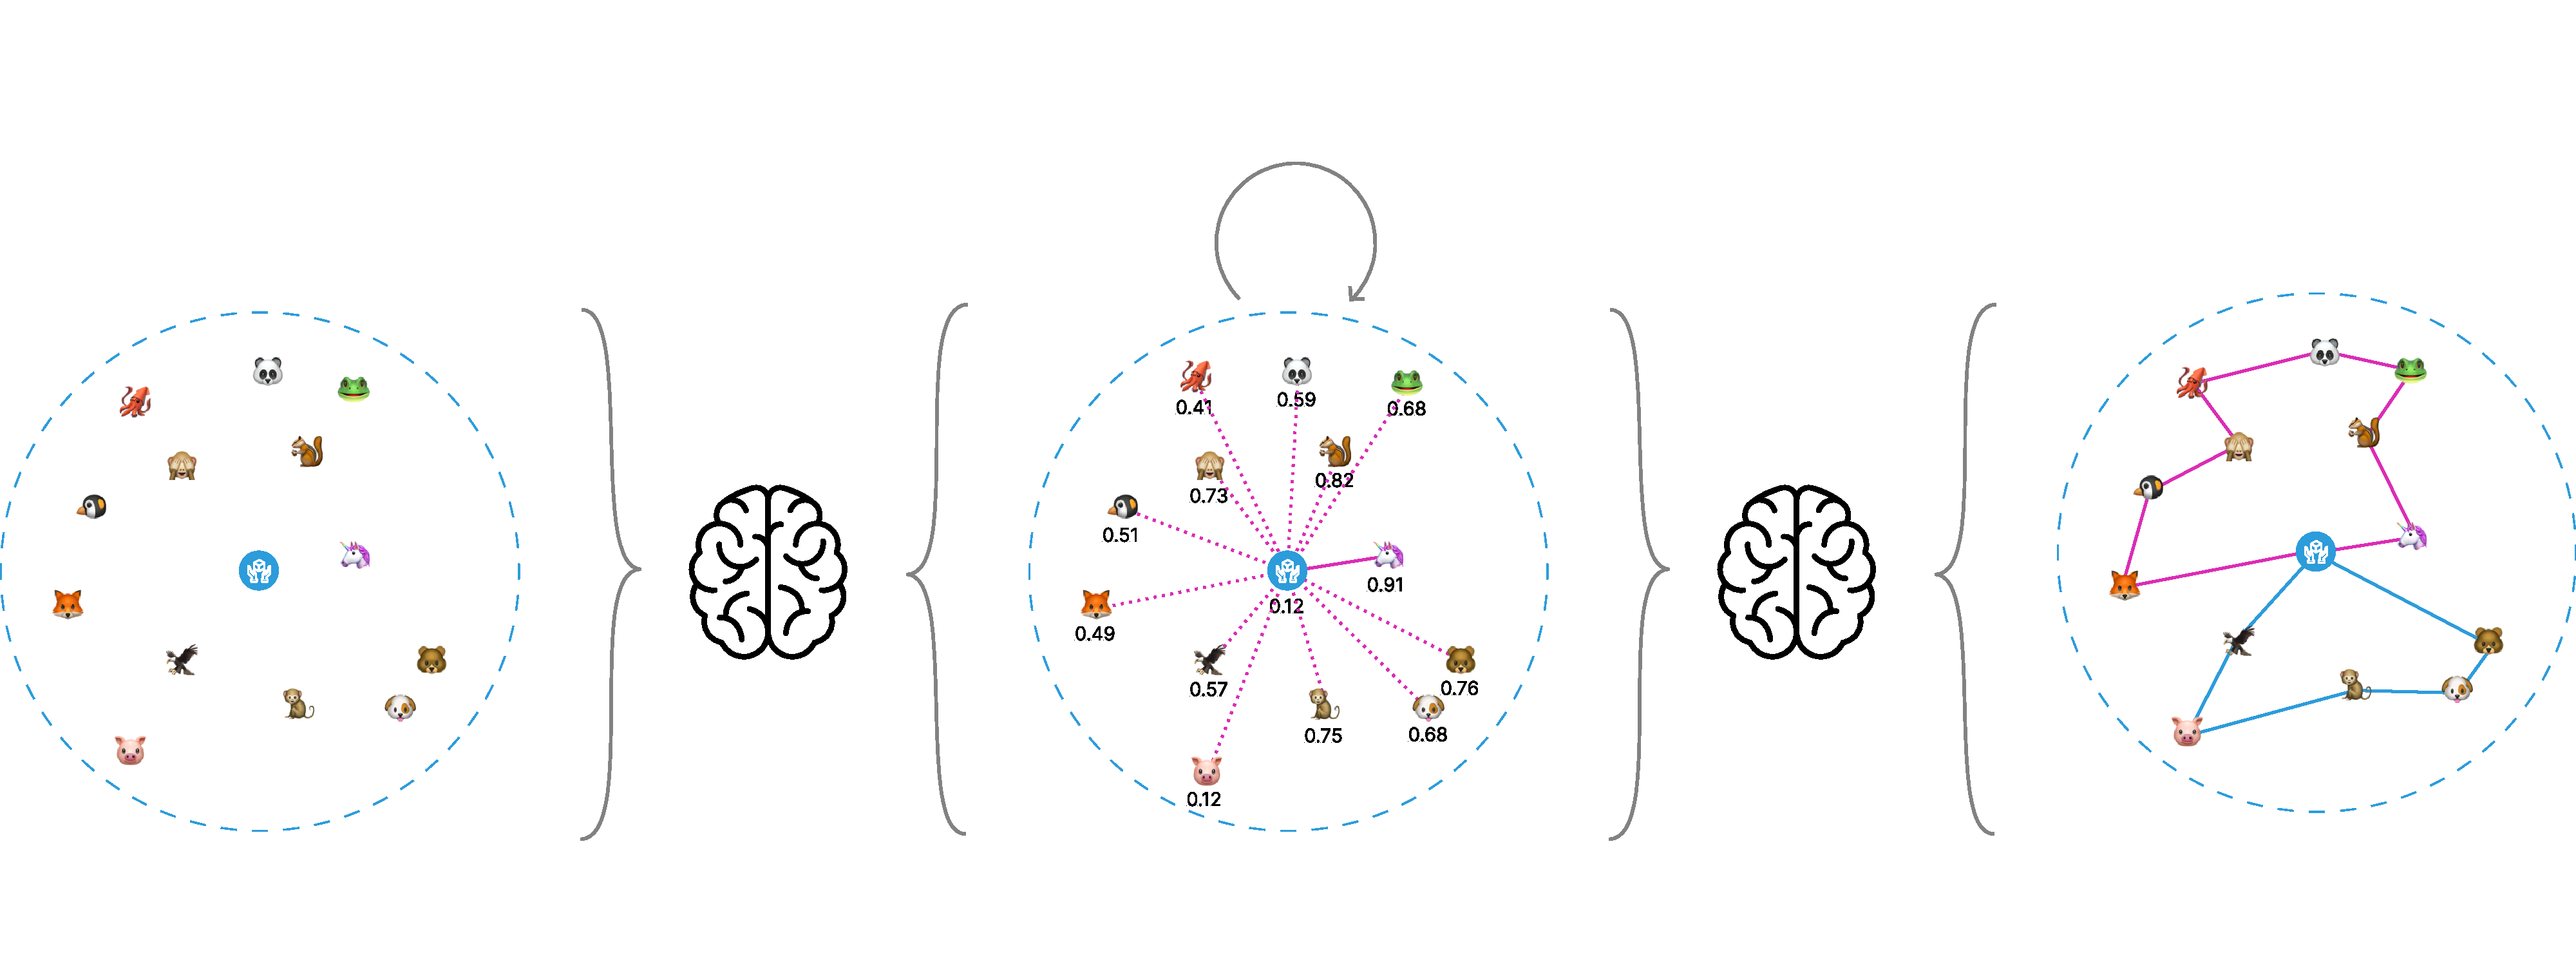
\includegraphics[width=1.0\textwidth]{resources/vrptw-ai/attention-route-diagram.pdf}
        \caption{High-level concept behind the used method.}
        \label{fig:attention-route-diagram}
    \end{figure}

    \subsection{Model Architecture}\label{vrptw-model}
    The model architecture \cite{attention-route} leveraging recent advancements in attention mechanism is here extended by the time window constraint. The model is built upon transformers \ref{transformer}, graph attention network \ref{graph-attention-network}, and reinforcement learning \ref{rl}. The network structure is encoder-decoder that fits well for solving sequential decision problems. The structural input instance is extracted by the encoder \ref{vrptw-encoder} and then the solution is incrementally constructed by the decoder \ref{vrptw-decoder}.
    
    The \gls{vrptw} input instance is consisted from:
    \begin{itemize}\label{input-data}
        \item $X = \{x_1, \cdots, x_n\}$ where $x_i$ is two-dimensional coordinates in the euclidean space.
        \item $x_0$ is the location of depot.
        \item $D = \{d_1, \cdots, d_n\})$ is the demand capacity for each of the locations.
        \item $T = \{(e_1, l_1), \cdots, (e_n, l_n)\})$ is time windows for each of the location where $e_i$ is the beginning and $l_i$ is the end of the considered time window.
    \end{itemize}
    
    The output is the solution of VRPTW instance and is represented as a permutation $\pi$ of locations $X \cup x_0$.
    \begin{itemize}
        \item $\pi = \{\pi_1, \cdots, \pi_T\} \in \{x_0, \cdots, x_n\})$ 
    \end{itemize}
    
    \subsubsection{Encoder}\label{vrptw-encoder}
    The encoder uses graph attention network \ref{graph-attention-network} to embed the node features to graph embedding. Then the decoder architecture is the same as the decoder of transformer \ref{transformer}. Typicaly, the decoder of transformer uses positional encoding \cite{positional-encoding} to embed the input, but in this case it has been replace with \gls{gat} \ref{graph-attention-network} since we deal with graph-based structure and the input order does not matter.
    
    The first step is to perform the initial embedding of input data \ref{input-data} via learned linear projections as in \gls{gat}. The $h_{i}^{l}$ represents the node embedding of layer $l \in \{0, \cdots, N\}$ (N=3).
    \begin{equation}
        \widetilde{x} = \text{concat}(X, D, T)
    \end{equation}
    \begin{equation}
        h_{i}^{0} = \begin{cases} W \widetilde{x}_i + b_i &\mbox{if } i > 0 \\ W \widetilde{x}_0 + b_0 & \mbox{if } n = 0 \end{cases}
    \end{equation}
    
    The node embeddings are updated via $N$ attention layers, each containing multi-head attention \ref{multi-head-attention} (M=8) and a fully connected feed-forward network with normalization. The structure is identical to transformer's encoder \ref{transformer} with additional support of graph structure \ref{graph-attention-network} as shown on Figure \ref{fig:encoder-diagram}.
    
    \begin{figure}[ht]
        \centering
        \includegraphics[width=1.0\textwidth]{resources/vrptw-ai/encoder-diagram.png}
        \caption{Encoder layers \cite{attention-route}}
        \label{fig:encoder-diagram}
    \end{figure}
    
    The equation \ref{encoder-qkv} calculates the query $Q$, key $K$ and value $V$ of multi-head attention layer using the node embeddings and weights $W_m^Q$, $W_m^Q$, and $W_m^Q$, respectively. The number of heads is represented by $m \in \{1, \cdots, M\}$ (M=8).
    
    \begin{equation}\label{encoder-qkv}
        \textbf{q}_{im}^l = W_m^Q h_i^(l-1), \textbf{k}_{im}^l = W_m^K h_i^(l-1), \textbf{v}_{im}^l = W_m^V h_i^(l-1)
    \end{equation}
    
    The query and key values are used in calculating the compatibility $u_{ijm}^l$ of node $i$ with a node $j$ \ref{mha-compatibility}. If node $i$ is not adjecnt to node $j$ then they are not compatible and the value is set to a large negative number.
    
    \begin{equation}\label{mha-compatibility}
        u_{ijm}^l = \begin{cases} q_{im}^l k_{jm}^l &\mbox{if $i$ adjacent to $j$} \\ -\infty &\mbox{otherwise} \end{cases}
    \end{equation}
    
    The attention score $a_{ijm}^l \in [0,1]$ is calculated using softmax from the compatibility values of nodes \ref{encoder-attention-score}
    
    \begin{equation}\label{encoder-attention-score}
        a_{ijm}^l = \dfrac{e^{u_{ijm}^l}}{\sum_{j'=0}^n e^{u_{ij'm}^l}}
    \end{equation}
    
    The transformed $h'_{im}^l$ \ref{h-prime} aggregates all attention scores across neighbour nodes, which is based on GAT \ref{graph-attention-network}. 

    \begin{equation}\label{h-prime}
        h'_{im}^l = \sum_{j=0}^n a_{ijm}^l v_{jm}^l
    \end{equation}
    
    Finally, we may calculate the multi-head attention \ref{transformer} for layer $l$ as a function of $\{h_1^{l-1}, \cdots, h_n^{l-1}\}$ through $h'_{im}^l$.
    
    \begin{equation}
        \text{MHA}_i^l(h_1^{l-1}, \cdots, h_n^{l-1}) = \sum_{m=1}^M W_{m}^O h'_{im}^l
    \end{equation}
    
    \begin{equation}
        \widetilde{h}_i = \text{BN}^l(h_i^{l-1} + \text{MHA}_i^l(h_1^{l-1}, \cdots, h_n^{l-1})))
    \end{equation}    
    \begin{equation}
        h_i^l = \text{BN}^l(\widetilde{h}_i + \text{FF}^l(\widetilde{h}_i))
    \end{equation}
    
    In the final layer, the encoder computes the aggregated embedding of the input graph as the mean of the final node embeddings.
    \begin{equation}
        h^N = \dfrac{1}{n} \sum_{i=1}^m h_i^N
    \end{equation}
    
    The output of the encoder's final layer is passed to the decoder, which is detailed in the next sections \ref{vrptw-decoder}.
    
    \subsubsection{Decoder}\label{vrptw-decoder}
    Decoder works sequentially through timestamps $t \in \{0, \cdots, n\}$, at each timestamp one node is selected to be visited based on partial route $\pi_{1:t-1}$. It is predicting the probability distribution over nodes according to the node embedding and context vector of the encoder \ref{vrptw-encoder}.
    
    \begin{figure}[ht]
        \centering
        \includegraphics[width=1.0\textwidth]{resources/vrptw-ai/decoder-diagram.png}
        \caption{Describes the decoder iteration in the construction of a solution. This diagram very nicely visualizes the process and it was used in the paper by Kool et al. \cite{attention-route}}
        \label{fig:encoder-diagram}
    \end{figure}
    
    The decoder uses a new context vector $h_{c}^{'}$ which represents the state \ref{rl} and it goes as follows:
    \begin{equation}\label{decode-state-vec}
        h_{c}^{'} = \begin{cases} \text{concat}(h_N; h_0^N; D_t) & \mbox{if } t = 0 \\ \text{concat}(h_N; h_{\pi_{1:t-1}}^N; D_t) & \mbox{if } t > 0 \end{cases}
    \end{equation}
    The state of $h_{c}^{'}$ is concatenation of $h_N$, the output of the encoder, $h_{\pi_{1:t-1}}^N$, the embedding of previous partial solution, and $D_t$, the remaining demand capacity of the vehicle.
    
    Due to the fact that the decoder architecture is transformer \ref{transformer}, the next layers are multi-head attentions which are responsible for choosing the next node to visit. This defines the system action \ref{rl}.
    
    The multi-head attention in the decoder is computed in a similar manner as in the decoder \ref{vrptw-encoder} with a little alternation.
    \begin{equation}
        q_{(c)m} = W_m^Q h_{c}^{'}, k_{jm} = W_m^K h_{j}^{N}, v_{jm} = W_m^V h_{j}^{N}
    \end{equation}
    
    \begin{equation}\label{compatibility-decoder}
        u_{(c)j} = \begin{cases} q_c^T k_j &\mbox{if }  d_j <= D_t \text{ and } x_j \notin \pi_{1:t-1} \\ -\infty &\mbox{otherwise} \end{cases}
    \end{equation}
    
    The equation \ref{compatibility-decoder} computes the compatibility score and performs a masking mechanism to mask the nodes which have already been visited during the partial route (besides depot $x_0$) and eliminates nodes where the vehicle capacity would overflow. If we would consider a time window as a hard constraint, the calculation of compatibility would have extended masking mechanism to show only nodes which correspond to the time $t$.
    
    \begin{equation}
        h'_{(c)m} = \sum_{j=0}^n softmax(u_{(c)j}) v_jm
    \end{equation}
        
    \begin{equation}
        h_{c} = \text{MHA}(h_{c}^{'}) = \sum_{m=1}^M W_{m}^O h'_{(c)m}
    \end{equation}
    
    In order to calculate the desired probability $p_{\theta}(\pi_t|X, \pi_{1:t-1})$, a logit layer. The final layer is a single-head attention.
    
    \begin{equation}
        q = W^Q h_c, k_j = W^K h_j^N
    \end{equation}
    
    \begin{equation}
        u_j = \begin{cases} C . \text{tanh}(q^T k_{c}) &\mbox{if }  d_j <= D_t \text{ and } x_j \notin \pi_{1:t-1} \\ -\infty &\mbox{otherwise} \end{cases}
    \end{equation}
    
    \begin{equation}\label{encoder-attention-score}
        p_i = p_{\theta}(\pi_t|X, \pi_{1:t-1}) = \dfrac{e^{u_j}}{\sum_{j'=0}^n e^{u_{j'}}}
    \end{equation}
    
    \subsection{Reinforcement Learning}\label{vrptw-rl}
    The model \ref{vrptw-model} takes \gls{vrptw} instance and outputs probability distribution over nodes $p_{\theta}(\pi|X)$ which is used to sample a full feasible route as a solution $\pi$. The instance of \gls{vrptw} $S$ is defined as concatenation of locations, demand capacity and time windows for each node, $S = [X, D, T]$.
    
    To train the model, we have to define a reward, respectively, a cost function. The model is trained using REINFORCE algorithm \ref{reinforce} as proposed by Kool et al. \cite{attention-route}. The algorithm is based on the computation of the policy gradient, which is defined as
    \begin{equation}\label{encoder-attention-score}
        \nabla_{\theta} \mathcal{L}(\theta|X) = \mathop{\mathbb{E}}[ \mathcal{L}(\pi|X) - b(X)) \nabla \ln \pi (\pi|X))]
    \end{equation}
    
        \subsubsection{VRPTW Cost}\label{vrptw-rl}
        For effectively solving \gls{vrptw}, the cost function is an integral part of a successfully trained model. In this thesis, we propose a new cost function to solve the vehicle routing problem with soft constrained time windows and demand capacity for each node.
        
        The cost function is ranking the given solution of \gls{vrptw} instance. It penalizes the solution based on the length of the routes, early and late visits, and unequal distribution of nodes across vehicles.
        
        For a given \gls{vrptw} instance $S$ and its solution $\pi$, we propose the cost function as follows:
        \newcommand{\norm}[1]{\left\lVert#1\right\rVert}
        \begin{equation}\label{vrptw-cost}
            \mathcal{L}(\pi|S) = dis_p(\pi, S) + t_p(\pi, S) + bal_p(\pi, S)
        \end{equation}
        \begin{equation}\label{distance-cost}
            dis_p(\pi, S) = \sum_{i=0}^N \norm{x_{\pi(i)} - x_{\pi(i+1)}}_2
        \end{equation}
        The equation \ref{distance-cost} calculates the length of all routes in Euclidean space.
        
        \begin{equation}\label{time-cost}
            t_p(\pi, S) = \sum_{i=0}^N (I_{e_i > \widetilde{t}_i} (e_i - \widetilde{t}_i) p_e + I_{l_i < \widetilde{t}_i} (\widetilde{t}_i - l_i) p_l)
        \end{equation}
        The equation \ref{time-cost} calculates the penalty for early or late arrival. The time of the visit for a given node $i$ is defined by vector $\widetilde{t}_i$. We assume that the travel speed is always identical and we approximate that one unit of distance equals to one unit of time. The vector $I$ behaves as a mask $I \in (0, 1)^n$ which represents if either early or late arrival occurred. The penalty for late arrival $p_l$ should be greater than for early arrival $p_e$ and finding the proper penalties will be empirically determined as a part of experiment chapter \ref{penalty-experiment}.
        
        \begin{equation}\label{balance-cost}
            bal_p(\pi, S) = \sigma([|R_0|, \cdots, |R_k|])
        \end{equation}
        The last subpart of the cost function is calculating balance cost \ref{balance-cost} that aims to evenly distribute the number of nodes in a route $R_i$ by minimizing its standard deviation. In logistics, we expect to utilize couriers evenly.
        
        \subsubsection{Training loop}\label{vrptw-loop}
        
        Pseudocode of the \gls{rl} system training loop is as follows
        
        \SetKwInput{KwInput}{Input} 
        \begin{algorithm}[H]
            \KwInput{Number of epoch $E$, steps per epoch $T$, batch size $B$} %significance $\alpha$
            \KwResult{Updated $\theta$ that maximises reward}
            
            Initialize $\theta$ at random\;
            \For{$epoche = 1, 2, \cdots, E$}{
                \For{$steps = 1, 2, \cdots, T$}{
                    Compute context embedding $h^N$ via decoder (\ref{vrptw-encoder});
                    
                    \For{$t = 1, 2, \cdots, N$}{
                        Calculate $p_{\theta}(\pi_t|X, \pi_{1:t-1})$ via encoder for $t$ (\ref{vrptw-decoder});
                        
                        Pick an action based on probability distribution;
                        
                        Update the state by visiting a new node;
                    }
                    
                    Compute reward $\mathcal{L}(\pi|S)$ (\ref{vrptw-cost});
                    
                    %Compute reward baseline;
                    
                    % $\nabla_{\theta} \mathcal{L} \gets \mathop{\mathbb{E}}[ \mathcal{L}(\pi|X) - b(X)) \nabla \ln \pi (\pi|X))]$;
                    
                    $\nabla_{\theta} \mathcal{L} \gets \mathop{\mathbb{E}}[ \mathcal{L}(\pi|X) \nabla \ln \pi (\pi|X))]$;
                    
                    $\theta \gets \text{Adam}(\theta, \nabla_{\theta} \mathcal{L})$;
                }
         }
         \caption{REINFORCE algorithm}
        \end{algorithm}
        
    
    \subsection{Integrating Duration Matrix}
    Real-world application of \gls{vrp} require to obtain the distance and duration matrix which represents the weighted transition between graph nodes. The duration between two locations is typically defined by the infrastructure and speed limits on a given route. Such a duration matrix is calculated using map data such as OpenStreetMap \cite{osm}.
    
    The neural network solving \gls{vrptw} learns to approximate the Euclidean distance between two given points. However, if we would integrate the duration matrix into the cost function of the model, the network would have to derive the duration between two points, which is an impossible task with the given model architecture. Moreover, the planning would be fixed to the location (city) on which the model was trained on.
    
    We propose an indirect integration of the duration matrix for the input instance. We may project the duration matrix into the node locations using multidimensional scaling \cite{mds} which would embed the duration information in a given 2D space.

    \chapter{Planning System}\label{system}

In this chapter, take a look at how the GoDeliver\footnote{\url{https://godeliver.co/}} system works and the integration of the \gls{vrptw} \gls{ai} planner.

\section{GoDeliver System}

The GoDeliver system is consisted of multiple services, each responsible for a given subproblem of the delivery process. The core of the system is GoDeliver service, which implements all system APIs and performs the basic CRUD\footnote{Create, read, update and delete} operation on our NoSQL database. The database stores information about business, delivery orders, couriers, and delivery plans. In the Figure \ref{fig:godeliver-system} is visualized the simplified architecture of GoDeliver system, it is especially oriented to show how the planning process works.

\begin{figure}[ht]
    \centering
    \includegraphics[width=1.0\textwidth]{resources/implementation/godeliver-system.png}
    \caption{GoDeliver System Architecture}
    \label{fig:godeliver-system}
\end{figure}

\subsection{Planning process}
The planning process is a complex operation which requires to work asynchronously because the planning of delivery orders is a time-consuming operation. The modern delivery planners have to support dynamic rescheduling and autonomously act upon the constantly changing environment.

The first part of the planning process is the creation of a delivery order, which is a request for delivery via API. The delivery order is saved in the database by GoDeliver Service with additional meta-data about the delivery state, etc. The database is monitored for a so-called \textit{trigger changes} which fires a replanning job via a distributed task queue Celery\footnote{\url{https://github.com/celery/celery}}. The \textit{trigger changes} are a list of actions such as creation of a new delivery order, changes in courier capacity, or a significant delay of delivery.

If such a replanning job is created, it is saved in Celery queue which is processed by GoDeliver Replanning Service \ref{fig:godeliver-system}. The replanning service loads a business configuration, delivery orders, and delivery plans from the database. It transforms the data into a generic structure which is accepted by our another service logistics planners that are solving the vehicle routing problem. The generic plan structure for the logistics planner freezes some delivery points which should not be considered by the planner since we do not want to change the current in-progress delivery points. This process is enabling us to perform the dynamic vehicle routing problem \ref{dynamic}.

Based on the business config, the desired vehicle routing solver is invoked via the logistics planner API. Usually, the planner takes the previous delivery plan and performs a heuristic algorithm like insertion heuristic which outputs an extended feasible plan. This plan is then improved by a local search algorithm to improve its cost function. Then the solution is processed by GoDeliver Replanning Service and saves the new delivery plans into the database.

\begin{figure}[ht]
    \centering
    \includegraphics[width=0.75\textwidth]{resources/implementation/godeliver-app.png}
    \caption{GoDeliver Driver App}
    \label{fig:godeliver-app}
\end{figure}

In the future, the proposed \gls{vrptw} \gls{ai} planner will be used instead of insertion heuristics because we expect the \gls{ai} planner will outperform the insertion heuristics. The downside is that \gls{ai} planner is not able to leverage on the previous solution, which can lead to drastic changes in the solution structure of the delivery plan. However, this side effect is not a blocker since couriers only see one current delivery point from the delivery plan via GoDeliver mobile app \ref{fig:godeliver-app}.

\subsection{Planning Requirements}
The GoDeliver objective is to provide the most advanced and versatile urban logistics system. The logistics cases are always different for individual businesses and in order to cover them all we require a flexible but yet powerful planning system. For a new planner to be successfully used in the production environment, we have defined the planner requirements which have to be supported \ref{tab:vrptw-feature}. 

In the table \ref{tab:vrptw-feature}, we have summarized the supported features of our proposed \gls{vrptw} \gls{ai} It does not support features such as Pick and Deliver, predefined number of vehicles, and distance matrix. The Pick and Delivery is possible to support by extending the model to support a heterogeneous fleet based on this paper by J. Li et. al \cite{pick-deliver-ai} which extends the masking mechanism and \gls{rl} state and action to support the pick and deliver constraints. Distance matrix could be indirectly supported by applying multidimensional scaling \cite{multidimensional-scaling} to project the distance matrix into Euclidean space which is supported by the model. To define a fixed number of vehicles for a given \gls{vrptw} instance is surprisingly more complicated, but we propose that it can be achieved by implementing the support of multiagent reinforcement learning \cite{multiagent-rl} where each agent is one vehicle.

\begin{table}
     \centering
     \begin{tabular}{||c | c||} 
     \hline
     Feature & Is supported? \\ [0.5ex] 
     \hline\hline
     Time windows & \checkmark \\ 
     \hline
     Soft constraint & \checkmark \\
     \hline
     Distance matrix & indirectly\footnote{Multidimensional scaling \cite{multidimensional-scaling}} \\
     \hline
     Pick and Deliver & - \\
     \hline
     Demand Capacity & \checkmark \\ 
     \hline
     Balanced load across vehicles & \checkmark \\ 
     \hline
     Predefined number of vehicles & - \\ [1ex] 
    \hline
    \end{tabular}
    \caption{VRPTW AI support of planner requirements}
    \label{tab:vrptw-feature}
\end{table}

\section{Tech Stack - VRPTW via Optimization}

The planners based on optimization heuristics are implemented in programming languages Python\footnote{\url{https://python.org/}} and Go\footnote{\url{https://golang.org/}} and our implemented metaheuristic uses the optimization framework OR-Tools.

\section{Tech Stack - VRPTW via AI}

The \gls{vrptw} planner via \gls{ai} is implemented in the programming language Python which is the most favorite programming language for any \gls{ai}-related project \cite{stack-overflow}. Besides it is easy language to get start with, it has many amazing \gls{ai} and data libraries such as Pandas, Numpy, Tensorflow or PyTorch.

Production implementation of neural network is developed with the use of deep learning frameworks. TensorFlow\footnote{\url{https://pytorch.org/}} and PyTorch\footnote{\url{https://pytorch.org/}} are the two most popular frameworks. It is an important decision which deep learning framework to choose if you plan to develop a production ready \gls{ml} pipeline.

\begin{figure}[ht]
    \centering
    \includegraphics[width=1.0\textwidth]{resources/implementation/dp-framework-trend.png}
    \caption{Google Trend of PyTorch (blue) vs Tensorflow (red)}
    \label{fig:dp-framework-trend}
\end{figure}

The Google Trends graph \ref{fig:dp-framework-trend} shows how TensorFlow was more popular in the past, but lately they have similar amount of search results. However, the majority of the new research papers are implemented via PyTorch \cite{pytorch-data}. It is due to the fact that PyTorch has a great and intuitive API based on Numpy\footnote{\url{https://numpy.org/}} operations and it is even slightly faster than TensorFlow.

In this thesis, we have decided to use PyTorch as our main deep learning framework.



    \chapter{Evaluation}
Choosing TW penalties
Model genealization
Training process - loss + used parametes
I1 vs Or-tools vs RL
    \begin{conclusion}
    The thesis objective was to explore if vehicle routing problem (\gls{VRP}) with time windows can be solved via machine learning.
\end{conclusion}

    
    % bibliography
    \bibliographystyle{prefs/iso690}
    \bibliography{ref}
    
    \appendix
    
    % acronyms
    \printglossaries
    
    % media contents
    \chapter{Media contents}\label{app:CDcontent}
    \begin{figure}
    	\dirtree{%
    		.1 readme.txt\DTcomment{the file with CD contents description}.
    		.1 data\DTcomment{the data files directory}.
    		.2 example\textunderscore sequence\DTcomment{the directory with example sequence from dataset}.
    		.3 *.jpg\DTcomment{the example images}.
    		.2 example\textunderscore sequence\textunderscore graphs\DTcomment{the directory of graphs of experiments}.
    		.3 *.png\DTcomment{the motion output graphs}.
    		.2 tracking\textunderscore example.mp4\DTcomment{the example video file}.
    		.1 src\DTcomment{the directory of source codes}.
    		.2 models\DTcomment{the directory of deep learning modules}.
    		.2 utils\DTcomment{the directory of helper modules}.
    		.2 *.py\DTcomment{the Python source files}.
    		.1 text\DTcomment{the thesis text directory}.
    		.2 thesis\DTcomment{the directory of \LaTeX{} source codes of the thesis}.
    		.2 thesis.pdf\DTcomment{the Diploma thesis in PDF format}.
    	}
    \end{figure}
    

\end{document}
